\documentclass[11pt,a4paper]{article}

\usepackage[margin=2.2cm]{geometry}
\usepackage{graphicx}
\usepackage{booktabs}
\usepackage{multirow}
\usepackage{amsmath}
\usepackage{float}
\usepackage[font=small,labelfont=bf]{caption}
\usepackage{xcolor}
\usepackage{tikz}
\usetikzlibrary{positioning,arrows.meta,shapes.geometric}
\usepackage[colorlinks=true,linkcolor=blue!60!black,citecolor=blue!60!black,urlcolor=blue!60!black]{hyperref}
\usepackage{enumitem}
\setlist{itemsep=2pt,topsep=4pt}

\newcommand{\best}[1]{\textbf{#1}}

\begin{document}

% ---------------------------------------------------------------- title page
\begin{titlepage}
\centering
{\scshape\LARGE International Institute of Information Technology\\[4pt] Hyderabad, India\par}
\vspace{1.6cm}
\rule{\linewidth}{0.6pt}\\[10pt]
{\Large\bfseries Reproducing and Extending a Hybrid Ensemble Model for\\[4pt]
APT Attack Detection: How Much of the Reported Performance Survives?\par}
\rule{\linewidth}{0.6pt}\\[18pt]
{\large Interim Project Report\par}
\vspace{6pt}
{\large Research in Information Security\par}
\vspace{1.4cm}
{\large Replication of:\par}
\vspace{4pt}
{\itshape Saini, Bhat Kasaragod, Prakasha \& Das (2023). ``A hybrid ensemble machine learning model for
detecting APT attacks based on network behavior anomaly detection.''\\
Concurrency and Computation: Practice and Experience, 35(28), e7865.\par}
\vspace{1.8cm}
{\large Submitted by\par}
\vspace{6pt}
\begin{tabular}{ll}
\toprule
Name & Roll Number \\
\midrule
Achyutananda Sahoo & [roll number] \\
{[team member]} & [roll number] \\
{[team member]} & [roll number] \\
\bottomrule
\end{tabular}
\vfill
{\large M.Tech in Computer Science and Information Security\par}
\vspace{4pt}
{\large Monsoon Semester 2026\par}
\end{titlepage}

\tableofcontents
\newpage

% ---------------------------------------------------------------- abstract
\begin{abstract}
\noindent
Saini et al.\ (2023) propose a ``hybrid'' ensemble of Random Forest (RF) and XGBoost, combined by averaging
predicted probabilities, for detecting Advanced Persistent Threat (APT) traffic, and report accuracies of
98.92\%, 99.91\%, 99.24\% and 97.11\% on CSE-CIC-IDS2018, CIC-IDS2017, NSL-KDD and UNSW-NB15. We reproduce
the full pipeline (cleaning, per-file stratified sampling, Pearson and mutual-information feature selection,
SMOTE-Tomek balancing, five baselines and the hybrid) on all four datasets, and add two extensions the paper
names as future work: a \emph{stacked} hybrid in which a trained meta-learner combines RF, XGBoost and an LSTM,
and an FT-Transformer as a modern tabular deep model.

On three of the four datasets our reproduction lands within 0.36 accuracy points of the paper, with a lower
false-positive rate on all three. UNSW-NB15 is the exception (91.33\% vs.\ 97.11\%); keeping the 40\% duplicate
rows that we remove closes about half of that gap. We also find that the hybrid's advantage over plain XGBoost
is negligible (on CIC-IDS2017 it is a single test flow out of 14{,}771), that the stacked hybrid makes
\emph{exactly} the same predictions as simple averaging on CIC-IDS2017 because the meta-learner ignores the
LSTM, and that the FT-Transformer trails the tree ensembles by 0.2--0.9 points while giving the lowest
false-positive rate on UNSW-NB15. While reproducing we reverse-engineered an undocumented 2\% sampling step for
CIC-IDS2017 and documented several internal inconsistencies in the paper. We close with a roadmap for a
leakage-free evaluation that tests how much of the reported performance survives.
\end{abstract}

% ---------------------------------------------------------------- 1 intro
\section{Introduction}

\subsection{Background}
An Advanced Persistent Threat (APT) is a long-running, targeted intrusion: attackers gain a foothold, move
laterally and exfiltrate data slowly while blending in with normal traffic. Signature-based defences such as
antivirus, firewalls and rule-based IDSs miss such activity because it rarely matches a known pattern.
Network behaviour anomaly detection (NBAD) instead learns what normal traffic looks like and flags deviations,
and machine learning is the usual tool for learning that boundary from labelled flow records.

\subsection{The paper being reproduced}
Saini et al.\ \cite{saini2023} evaluate ten classical classifiers and three deep models on four public intrusion
datasets, and propose a hybrid of RF and XGBoost whose predicted probabilities are averaged using the
\texttt{SimpleClassifierAggregator} of the \texttt{combo} library. Their pipeline merges all attack types into a single
``anomaly'' class (binary classification), balances the classes with SMOTE-Tomek, selects features with Pearson
correlation followed by mutual information, and explains the model with SHAP. The hybrid reports the highest
accuracy on every dataset. The paper's own Conclusion names combining machine-learning and deep-learning models,
including LSTMs, as future work.

\subsection{Our contributions}
\begin{enumerate}
  \item \textbf{A complete, open reproduction} of the paper's pipeline on all four datasets, run as a single
        configurable codebase (Section~\ref{sec:method}).
  \item \textbf{Reverse-engineered, undocumented details}, most notably a 2\% stratified sample of CIC-IDS2017 that
        the paper never mentions but that its own class counts reveal exactly (Section~\ref{sec:sampling}).
  \item \textbf{An explanation of the one large gap} (UNSW-NB15) through a duplicate-row ablation
        (Section~\ref{sec:unsw}).
  \item \textbf{Two extensions the paper proposes but does not evaluate}: a stacked ensemble of RF, XGBoost and an LSTM
        with a trained meta-learner, and an FT-Transformer (Section~\ref{sec:novel}).
  \item \textbf{A critical reading} of the paper's evaluation, listing verifiable internal inconsistencies and a
        roadmap for a leakage-free re-evaluation (Sections~\ref{sec:issues} and~\ref{sec:future}).
\end{enumerate}

% ---------------------------------------------------------------- 2 related work
\section{Related Work}
\begin{itemize}
  \item \textbf{Ensembles for intrusion detection.} RF and gradient-boosted trees are consistently strong on
        flow-feature datasets such as CIC-IDS2017 and CSE-CIC-IDS2018; the paper's comparison table cites
        D'hooge et al.\ \cite{dhooge2020}, who also showed that models trained on one CIC dataset transfer poorly to
        the other.
  \item \textbf{Deep learning on tabular data.} Gorishniy et al.\ \cite{gorishniy2021} introduced the
        FT-Transformer, which turns each feature into a token and applies self-attention; Grinsztajn et al.\
        \cite{grinsztajn2022} showed that tree ensembles still tend to outperform deep models on
        medium-sized tabular data.
  \item \textbf{Dataset quality.} Engelen et al.\ \cite{engelen2021} documented labelling and flow-construction
        errors in CIC-IDS2017, which matter when accuracies are reported to two decimal places.
  \item \textbf{Stacking.} Stacked generalisation \cite{wolpert1992} trains a meta-learner on out-of-fold base-model
        predictions and is the standard alternative to fixed-weight averaging.
\end{itemize}

% ---------------------------------------------------------------- 3 datasets
\section{Datasets and Exploratory Analysis}
\label{sec:data}

All four datasets from the paper were used. Before building the cleaning step we ran an exploratory analysis of
the \emph{raw} files (one notebook per dataset) to decide, from evidence, what the cleaning must handle.

\begin{table}[H]
\centering
\caption{Datasets as used in this study. ``Used rows'' is after sampling and duplicate removal.}
\label{tab:datasets}
\small
\begin{tabular}{lrrrrl}
\toprule
Dataset & Raw files & Raw rows & Raw attack share & Used rows & Sampling \\
\midrule
NSL-KDD          & 2  & 148{,}517      & 48.1\% & 147{,}888 & none \\
UNSW-NB15        & 2  & 257{,}673      & 63.9\% & 154{,}098 & none \\
CIC-IDS2017      & 8  & $\approx$2.83M & $\approx$19.7\% & 49{,}235  & 2\% per file \\
CSE-CIC-IDS2018  & 10 & 16.23M         & 16.9\% & 30{,}838  & 0.2\% per file \\
\bottomrule
\end{tabular}
\end{table}

\subsection{Findings that shaped the cleaning step}
\begin{itemize}
  \item \textbf{Class imbalance differs sharply.} NSL-KDD and UNSW-NB15 are close to balanced (48\% and 64\% attack),
        whereas the two CIC datasets are 17--20\% attack, so SMOTE-Tomek matters most for them
        (Figure~\ref{fig:eda2018}).
  \item \textbf{CSE-CIC-IDS2018:} the header row is repeated 59 times inside the data (these rows would otherwise be
        labelled as attacks); \texttt{Flow Byts/s} and \texttt{Flow Pkts/s} contain the literal text
        \texttt{Infinity}; and one 3.9\,GB file (\texttt{02-20-2018.csv}) carries four extra identifier columns
        (Flow ID, Src IP, Src Port, Dst IP) that the paper also drops.
  \item \textbf{CIC-IDS2017:} column names carry leading spaces (\texttt{' Label'}); eight columns are constant; the
        same two rate columns contain infinities; and 65 feature pairs are correlated above 0.9.
  \item \textbf{UNSW-NB15:} \texttt{label} is already binary and \texttt{attack\_cat} names the attack family, so both
        must be excluded from the features (a leakage trap); 40\% of rows are exact duplicates.
  \item \textbf{NSL-KDD:} no header row, three text categoricals (\texttt{protocol\_type}, \texttt{service},
        \texttt{flag}), one constant column and 13 highly correlated pairs.
\end{itemize}

\begin{figure}[H]
\centering
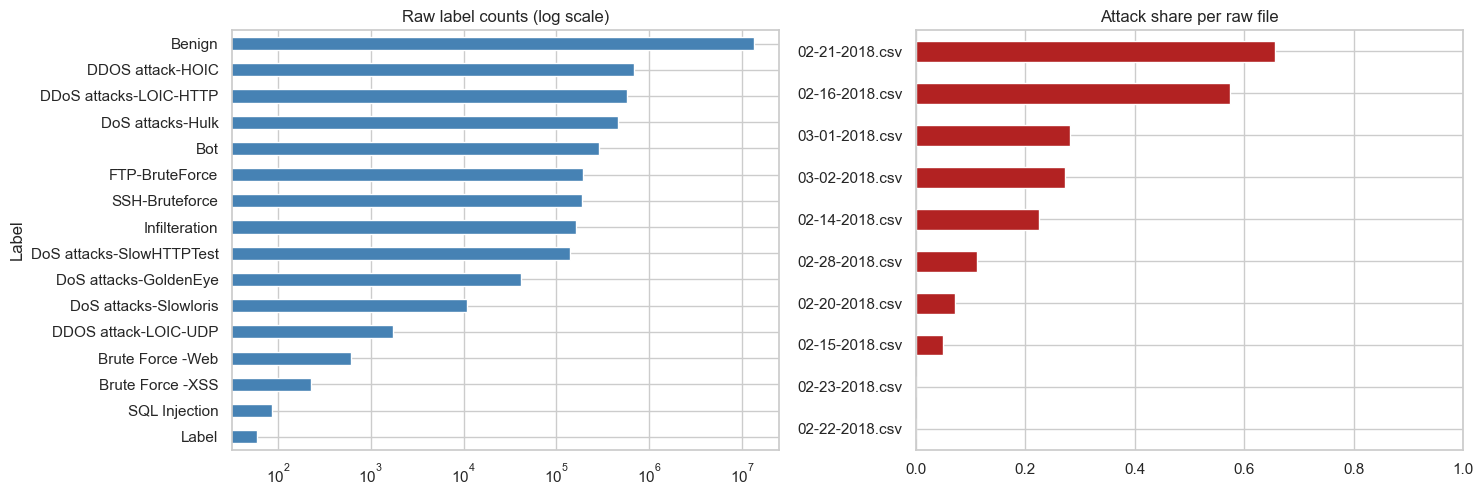
\includegraphics[width=\linewidth]{figures/eda_cse_cic_ids2018_classes.png}
\caption{CSE-CIC-IDS2018 raw labels (exact counts over all 16.2M flows). Left: label counts on a log scale; the
``Label'' bar is the header row repeated inside the data. Right: attack share per daily file, which varies from
0\% to 66\%. This variation is why the paper samples each file separately, preserving each day's mix.}
\label{fig:eda2018}
\end{figure}

% ---------------------------------------------------------------- 4 method
\section{Methodology}
\label{sec:method}

\subsection{Pipeline overview}
Figure~\ref{fig:pipeline} shows the pipeline. Every step is shared by all four datasets; dataset-specific choices
(label column, benign value, columns to drop, categoricals, sampling rate) live in a single configuration file.

\begin{figure}[H]
\centering
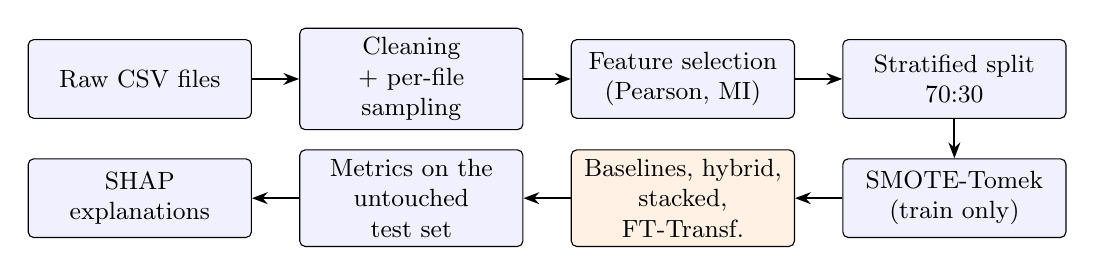
\begin{tikzpicture}[
  node distance=5mm and 6mm,
  box/.style={draw, rounded corners=2pt, fill=blue!6, align=center, font=\small, minimum height=10mm, text width=26mm},
  model/.style={box, fill=orange!10},
  arrow/.style={-{Stealth[length=2mm]}, thick}]
\node[box] (raw) {Raw CSV files};
\node[box, right=of raw] (clean) {Cleaning\\+ per-file sampling};
\node[box, right=of clean] (fs) {Feature selection\\(Pearson, MI)};
\node[box, right=of fs] (split) {Stratified split\\70:30};
\node[box, below=of split] (bal) {SMOTE-Tomek\\(train only)};
\node[model, left=of bal] (models) {Baselines, hybrid,\\stacked, FT-Transf.};
\node[box, left=of models] (eval) {Metrics on the\\untouched test set};
\node[box, left=of eval] (shap) {SHAP\\explanations};
\draw[arrow] (raw) -- (clean);
\draw[arrow] (clean) -- (fs);
\draw[arrow] (fs) -- (split);
\draw[arrow] (split) -- (bal);
\draw[arrow] (bal) -- (models);
\draw[arrow] (models) -- (eval);
\draw[arrow] (eval) -- (shap);
\end{tikzpicture}
\caption{Our pipeline. Unlike the paper, balancing is applied to the training split only, so the test set keeps
the natural class distribution.}
\label{fig:pipeline}
\end{figure}

\subsection{Preprocessing}
\begin{enumerate}
  \item \textbf{Load and clean labels.} Column names are stripped of whitespace, repeated header rows are removed,
        and all attack types are collapsed into one class: 0 = benign/normal, 1 = attack, exactly as in the paper.
  \item \textbf{Per-file stratified sampling.} CSE-CIC-IDS2018 is sampled at 0.2\% per file (stated in the paper).
        CIC-IDS2017 is sampled at 2\% per file (\emph{not} stated in the paper, see Section~\ref{sec:sampling}).
  \item \textbf{Drop identifiers.} \texttt{Timestamp} is dropped everywhere (as in the paper), plus Flow ID and
        IP/port identifiers for 2018, and \texttt{id} and \texttt{attack\_cat} for UNSW-NB15.
  \item \textbf{Encode categoricals.} NSL-KDD and UNSW-NB15 text categoricals are label-encoded; the 2018
        \texttt{Protocol} column is one-hot encoded, because the paper's feature list contains
        \texttt{Protocol\_6} and \texttt{Protocol\_0}.
  \item \textbf{Remove duplicates, coerce to numbers, replace infinities.} Values are converted to numbers
        \emph{before} infinities are replaced, since the text \texttt{Infinity} only becomes a real infinity on
        conversion.
\end{enumerate}

\subsection{Feature selection}
Following the paper: zero-variance features are removed, then for every pair of features correlated above 0.9
one is dropped, then the 30 features with the highest mutual information with the label are kept.
Table~\ref{tab:fs} compares the counts. In that first run on CSE-CIC-IDS2018, 27 of our 30 selected features also appear in the
paper's top 30 (its Figure~8), and the leading features agree: \texttt{Init Fwd Win Byts}, \texttt{Dst Port},
\texttt{Fwd Pkt Len Max} and \texttt{Fwd Pkt Len Mean}.

\begin{table}[H]
\centering
\caption{Feature counts through selection (non-constant $\rightarrow$ after correlation pruning $\rightarrow$ kept).
Our CIC counts come from the first preparation run (CIC-IDS2017 before the Wednesday file was added;
CSE-CIC-IDS2018 before \texttt{Protocol} was one-hot encoded).}
\label{tab:fs}
\small
\begin{tabular}{lcc}
\toprule
Dataset & Ours & Paper \\
\midrule
NSL-KDD         & 40 $\rightarrow$ 33 $\rightarrow$ 30 & not reported \\
UNSW-NB15       & 42 $\rightarrow$ 32 $\rightarrow$ 30 & not reported \\
CIC-IDS2017     & 70 $\rightarrow$ 38 $\rightarrow$ 30 & ? $\rightarrow$ 36 $\rightarrow$ 30 \\
CSE-CIC-IDS2018 & 70 $\rightarrow$ 36 $\rightarrow$ 30 & 71 $\rightarrow$ 40 $\rightarrow$ 30 \\
\bottomrule
\end{tabular}
\end{table}

\subsection{Reverse-engineering the CIC-IDS2017 sampling}
\label{sec:sampling}
The paper describes sampling only for CSE-CIC-IDS2018, yet its CIC-IDS2017 class table (Table~4) totals about
56{,}600 rows, far below the $\approx$2.83M rows in the dataset. Dividing each of the paper's class counts by the
raw count reveals the step (Table~\ref{tab:sampling}): every attack class is exactly 2\% of its raw count.
The authors therefore took an undocumented 2\% stratified sample, and we do the same. This check also showed that
one of our files (Wednesday, the DoS day) was initially missing; it was added before the final runs.

\begin{table}[H]
\centering
\caption{The paper's CIC-IDS2017 counts divided by the raw counts.}
\label{tab:sampling}
\small
\begin{tabular}{lrrr}
\toprule
Class & Raw count & Paper (Table 4) & Ratio \\
\midrule
PortScan    & 158{,}930 & 3{,}179 & 2.00\% \\
DDoS        & 128{,}027 & 2{,}561 & 2.00\% \\
FTP-Patator & 7{,}938   & 159     & 2.00\% \\
SSH-Patator & 5{,}897   & 118     & 2.00\% \\
Bot         & 1{,}966   & 39      & 1.98\% \\
\bottomrule
\end{tabular}
\end{table}

\subsection{Balancing, splitting and models}
Data are split 70:30 with stratification (the paper's text says 70:30; its pseudocode says 80:20). SMOTE-Tomek is
then fitted on the \textbf{training split only}. The paper balances \emph{before} splitting, which places synthetic
samples interpolated from test rows into training; we avoid that leak deliberately, so our test sets keep their
natural class mix.

\paragraph{Reproduction models.} Decision Tree, Logistic Regression and MLP (both with feature standardisation,
which the paper's methodology figure includes), Random Forest (200 trees), XGBoost (200 trees), and the paper's
\textbf{averaging hybrid}: the mean of RF and XGBoost predicted probabilities, thresholded at 0.5, which is what
\texttt{combo}'s average aggregator computes. We evaluate a representative five baselines rather than all
thirteen of the paper's models.

\subsection{Extensions}
\label{sec:novel}
\paragraph{Stacked hybrid (RF + XGBoost + LSTM).} The paper's hybrid uses a fixed 50/50 average. Stacked
generalisation instead \emph{learns} how to combine models: out-of-fold probabilities from three-fold
cross-validation of each base model train a logistic-regression meta-learner, and the base models are then refit on
the full training set. The deep base learner is an LSTM (hidden size 32, 12 epochs), which follows the paper's
future-work suggestion; each flow's 30 features are fed as a length-30 sequence.

\paragraph{FT-Transformer.} Following Gorishniy et al.\ \cite{gorishniy2021}: each feature gets its own learned
linear embedding (a ``token''), a \texttt{[CLS]} token is prepended, three pre-norm Transformer blocks (token width
64, 8 heads) mix the tokens, and a head reads the \texttt{[CLS]} output. Inputs are quantile-normalised; training
uses AdamW (learning rate $10^{-4}$) with early stopping on a 10\% validation split, up to 40 epochs.

\subsection{Metrics and implementation}
Accuracy, precision, recall, F1, false-positive rate (FPR), false-negative rate (FNR) and ROC-AUC from predicted
probabilities are reported on the held-out test set. All randomness is seeded (\texttt{random\_state=42}); two
repeated runs produced identical numbers. The code is in Python (scikit-learn, imbalanced-learn, XGBoost, PyTorch,
SHAP); experiments ran on Kaggle, partly with an NVIDIA T4 GPU.

% ---------------------------------------------------------------- 5 results
\section{Results}

\subsection{Reproduction of the paper's hybrid}
\begin{table}[H]
\centering
\caption{The paper's averaging hybrid: reported vs.\ reproduced. Values in \%, except AUC. The paper's AUCs are
read from its ROC figures (none was transcribed for CSE-CIC-IDS2018).}
\label{tab:repro}
\small
\begin{tabular}{llcccccc}
\toprule
Dataset & Source & Accuracy & Precision & Recall & F1 & FPR & AUC \\
\midrule
\multirow{2}{*}{NSL-KDD}         & Paper & 99.24 & 99.28 & 99.09 & 99.18 & 0.62 & 0.992 \\
                                 & Ours  & 99.60 & 99.64 & 99.53 & 99.59 & 0.33 & 0.9999 \\
\midrule
\multirow{2}{*}{UNSW-NB15}       & Paper & 97.11 & 95.89 & 99.04 & 97.44 & 5.29 & 0.969 \\
                                 & Ours  & 91.33 & 89.11 & 91.67 & 90.37 & 8.94 & 0.980 \\
\midrule
\multirow{2}{*}{CSE-CIC-IDS2018} & Paper & 98.92 & 99.47 & 98.35 & 98.90 & 0.52 & -- \\
                                 & Ours  & 98.59 & 97.66 & 92.59 & 95.06 & 0.38 & 0.976 \\
\midrule
\multirow{2}{*}{CIC-IDS2017}     & Paper & 99.91 & 99.88 & 99.95 & 99.91 & 0.12 & 0.999 \\
                                 & Ours  & 99.86 & 99.60 & 99.74 & 99.67 & 0.10 & 0.9999 \\
\bottomrule
\end{tabular}
\end{table}

On NSL-KDD, CSE-CIC-IDS2018 and CIC-IDS2017 the reproduced accuracy is within 0.36 points of the paper, and our
false-positive rate is lower on all three. Our lower 2018 recall and F1 are expected: our test set keeps the natural
85/15 benign-to-attack mix, whereas the paper's appears to have been balanced before splitting, which inflates
recall. Per-model results for every dataset are in Appendix~\ref{app:full}; the paper's model ranking reproduces,
with tree ensembles on top and the hybrid best or within 0.01 points of the best model.

\subsection{The UNSW-NB15 gap and duplicate rows}
\label{sec:unsw}
UNSW-NB15 is the one dataset where we fall well short (91.33\% vs.\ 97.11\%). 40\% of its rows are exact duplicates;
we remove them, and the paper does not say whether it did. Keeping duplicates lets identical rows sit in both
training and test sets:

\begin{table}[H]
\centering
\caption{UNSW-NB15 with and without duplicate removal (averaging hybrid).}
\label{tab:unsw}
\small
\begin{tabular}{lccc}
\toprule
Setting & Accuracy & F1 & FPR \\
\midrule
Duplicates removed (ours)  & 91.33 & 90.37 & 8.94 \\
Duplicates kept (ablation) & 94.05 & 95.32 & 7.25 \\
Paper                      & 97.11 & 97.44 & 5.29 \\
\bottomrule
\end{tabular}
\end{table}

Keeping duplicates recovers 2.7 of the 5.8-point gap. The remainder is plausibly explained by balancing before the
split and by the paper's different, undescribed subset: its Table~6 lists about 81{,}000 records, while the official
partitions contain 257{,}673.

\subsection{Extensions: stacked hybrid and FT-Transformer}
All three models below were trained and tested on identical splits, so they compare directly.

\begin{table}[H]
\centering
\caption{Our extensions vs.\ the reproduced averaging hybrid. Accuracy and FPR in \%. Best of our three in bold.}
\label{tab:novel}
\small
\begin{tabular}{lcccccc}
\toprule
& \multicolumn{2}{c}{Averaging hybrid} & \multicolumn{2}{c}{Stacked (RF+XGB+LSTM)} & \multicolumn{2}{c}{FT-Transformer} \\
\cmidrule(lr){2-3}\cmidrule(lr){4-5}\cmidrule(lr){6-7}
Dataset & Acc. & FPR & Acc. & FPR & Acc. & FPR \\
\midrule
NSL-KDD         & \best{99.60} & \best{0.33} & \best{99.60} & 0.34 & 99.26 & 0.65 \\
UNSW-NB15       & \best{91.33} & 8.94 & \best{91.33} & 8.54 & 90.47 & \best{7.27} \\
CSE-CIC-IDS2018 & \best{98.59} & \best{0.38} & 98.57 & 0.43 & 98.42 & 0.59 \\
CIC-IDS2017     & \best{99.86} & \best{0.10} & \best{99.86} & \best{0.10} & 99.60 & 0.34 \\
\bottomrule
\end{tabular}
\end{table}

\begin{figure}[H]
\centering
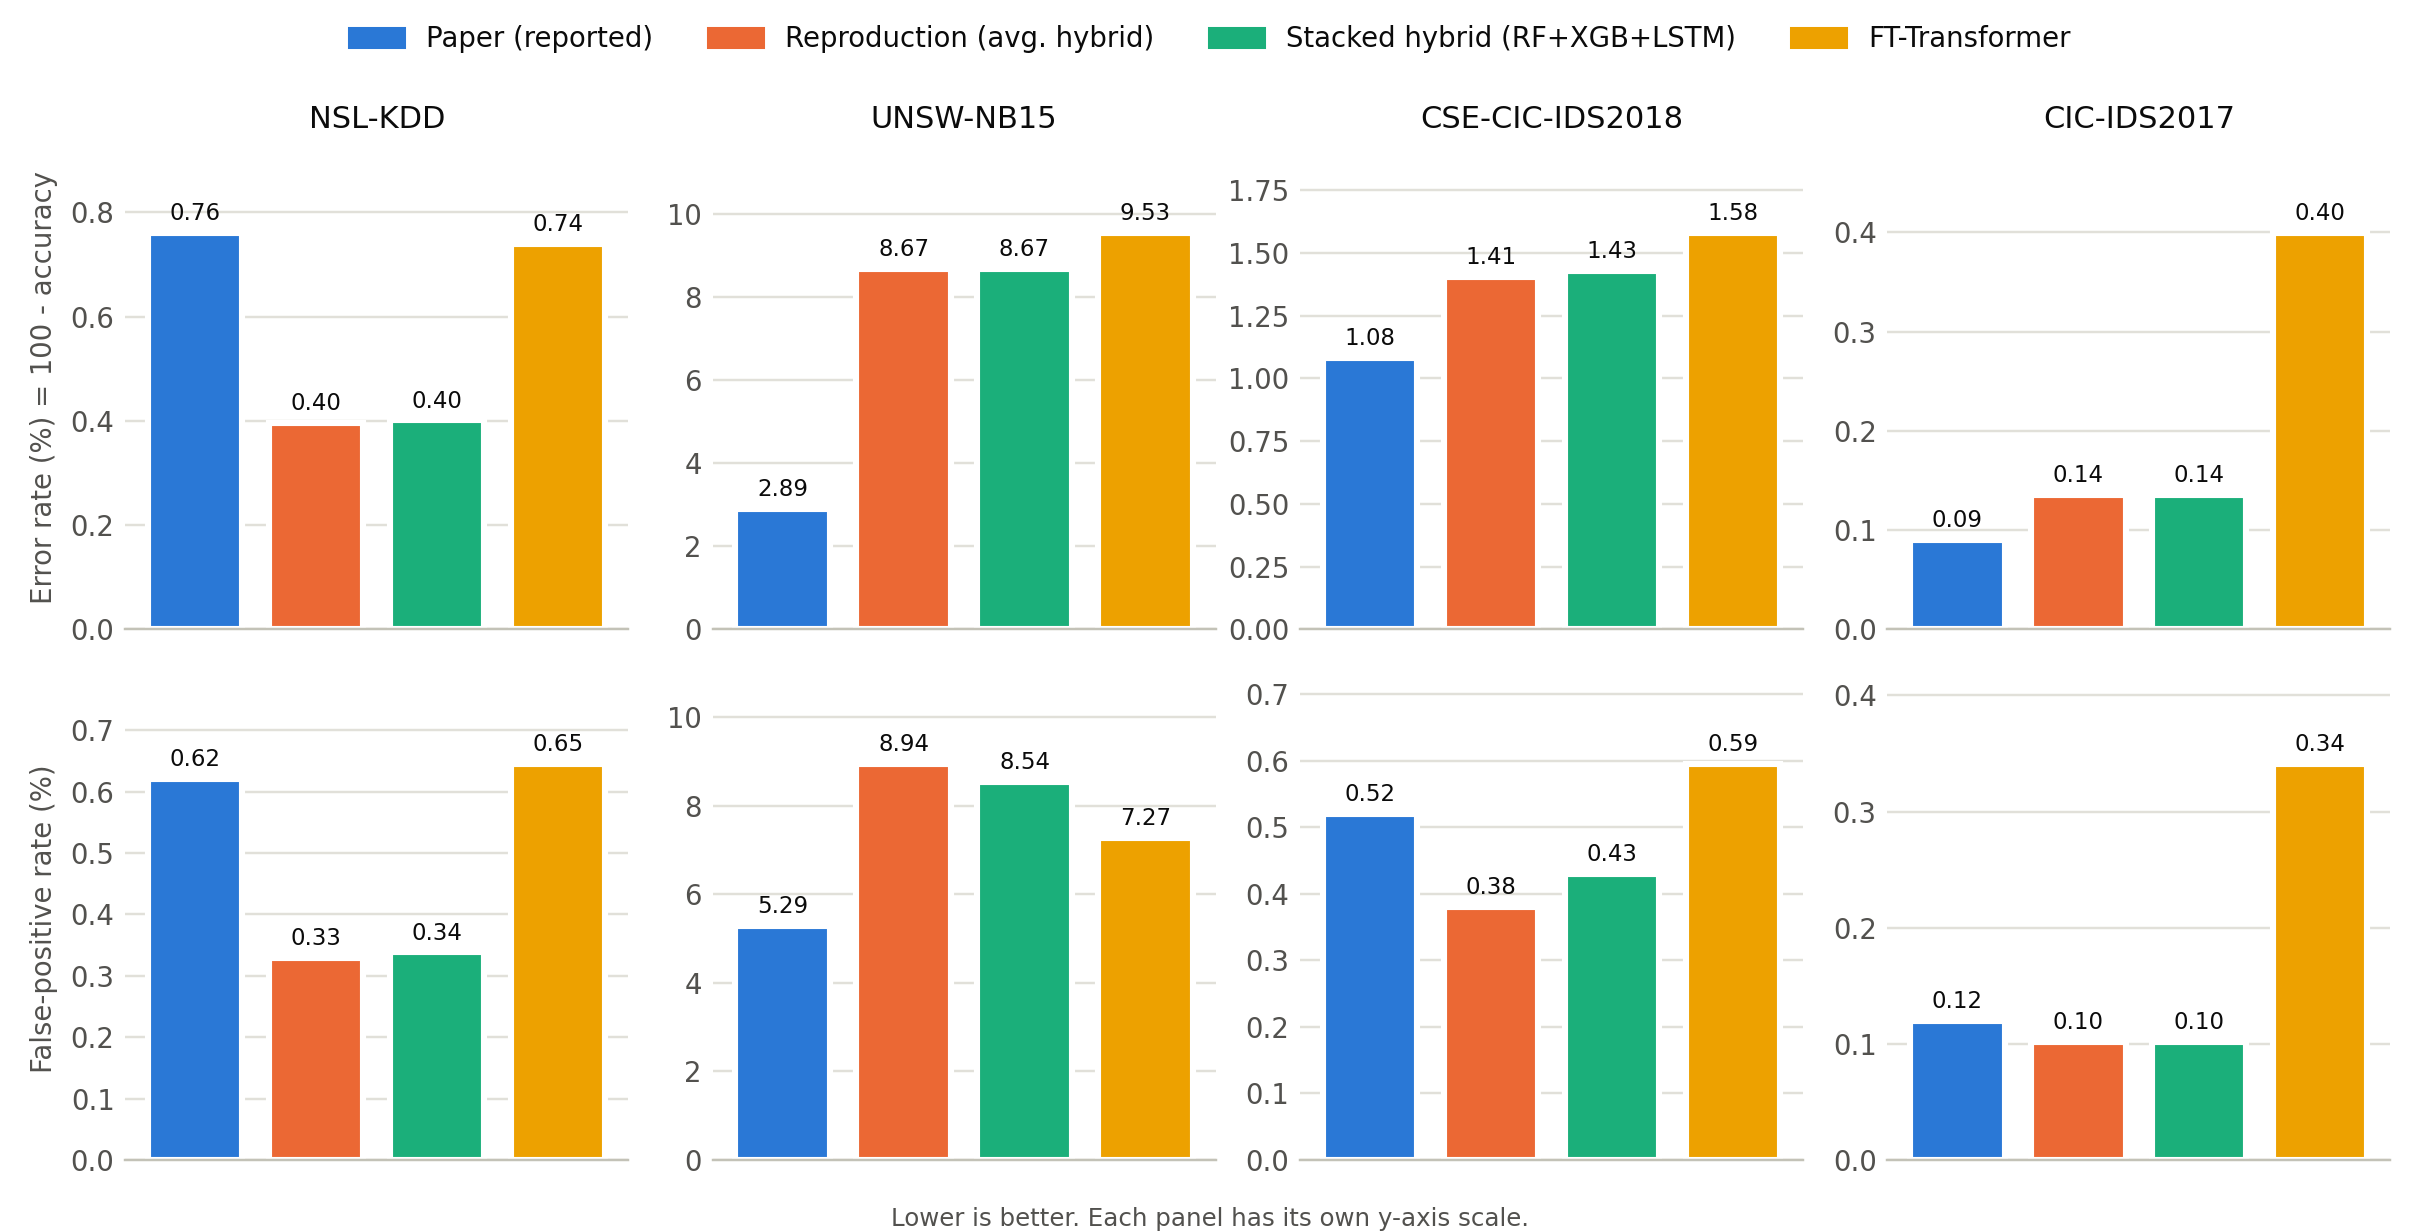
\includegraphics[width=\linewidth]{figures/results_error_fpr.png}
\caption{Error rate (100 $-$ accuracy) and false-positive rate for the paper's reported hybrid, our reproduction,
and our two extensions. Lower is better; each panel has its own scale.}
\label{fig:results}
\end{figure}

% ---------------------------------------------------------------- 6 discussion
\section{Discussion}

\subsection{The hybrid's advantage is negligible}
The paper's central claim, that the hybrid beats every other model, holds in our runs only by margins that no
single-seed experiment can distinguish from noise. On CIC-IDS2017 the hybrid scores 99.865\% and XGBoost alone
99.858\%: \emph{one} additional correct prediction out of 14{,}771 test flows. On NSL-KDD, XGBoost alone is marginally
ahead (99.61\% vs.\ 99.60\%). A claim of superiority needs repeated runs and a significance test, which the paper does
not report.

\subsection{Stacking collapses to averaging}
A trained combiner is strictly more expressive than a fixed average, yet the stacked hybrid never improves on it.
On CIC-IDS2017 its predictions are \emph{identical} to the averaging hybrid's (same accuracy, precision, recall, FPR
and FNR to every decimal place); only AUC differs, and it is slightly lower. This indicates that the meta-learner relies
almost entirely on RF and XGBoost and gives the LSTM little weight (its weights were not logged in these runs). The
LSTM is the weakest base model (training loss 0.12--0.22, unstable on
UNSW-NB15). This is expected: stacking gains come from base models that make \emph{different} errors, while RF and
XGBoost are highly correlated and the LSTM is weaker than both. There is also a design reason: an LSTM assumes a
meaningful order, but the ``sequence'' here is just the column order of one flow's features.

\subsection{FT-Transformer vs.\ tree ensembles}
The FT-Transformer is 0.2--0.9 points less accurate than the tree ensembles on every dataset, consistent with the
finding that trees still lead on medium-sized tabular data \cite{grinsztajn2022}. It does, however, give the lowest
false-positive rate on UNSW-NB15 (7.27\% vs.\ 8.94\%), meaning its errors differ from the trees'. That makes it a
better candidate than the LSTM for a stacked ensemble. Its validation loss was still falling at the 40-epoch cap on
three datasets, so these numbers are slightly pessimistic.

\subsection{Issues found in the paper}
\label{sec:issues}
While reproducing, we found the following issues, each verifiable from the paper itself:
\begin{itemize}
  \item \textbf{Balancing before splitting.} SMOTE-Tomek is applied to the whole dataset and the result is then
        split (p.~10), so synthetic samples derived from test rows enter training.
  \item \textbf{Undocumented sampling.} CIC-IDS2017 is sampled at exactly 2\% (Table~\ref{tab:sampling}), but the
        text describes sampling only for CSE-CIC-IDS2018.
  \item \textbf{Split ratio.} The text says 70:30; Algorithm~1 says 80:20.
  \item \textbf{Hyperparameters.} Algorithm~1 lists a learning rate of 1.0 and a maximum depth of 4 for the hybrid,
        which is unusual for XGBoost and would severely limit a Random Forest.
  \item \textbf{Identical deep-learning rows.} The CNN, ANN and MLP results are identical, to two decimals, in the
        NSL-KDD and UNSW-NB15 tables (Tables~9 and~10), although the datasets differ completely.
  \item \textbf{An impossible F1.} In the UNSW-NB15 table, logistic regression has precision 93.84 and recall 99.66,
        which implies F1 $\approx$ 96.66, yet the table reports 99.66.
  \item \textbf{Hard-label ROC curves.} The ROC curves (e.g.\ Figures~20, 22 and 24) consist of two straight
        segments, which is what a curve drawn from hard 0/1 predictions looks like; the reported AUC would then equal
        balanced accuracy rather than a ranking measure.
  \item \textbf{No variance.} No cross-validation, repeated seeds or significance tests are reported, although many
        claimed improvements are below 0.3 points.
\end{itemize}

% ---------------------------------------------------------------- 7 limitations
\section{Limitations of This Study}
We hold our own work to the same standard:
\begin{itemize}
  \item \textbf{Feature selection sees the whole dataset.} Like the paper, correlation pruning and mutual-information
        ranking run before the train/test split, which leaks a little test information into feature choice.
  \item \textbf{NSL-KDD split.} We merge the official KDDTrain+ and KDDTest+ files and split randomly (as the paper
        appears to), instead of using the official test set, which contains attack types absent from training and
        is known to be much harder.
  \item \textbf{Single seed.} All results come from one seeded split; we report no confidence intervals.
  \item \textbf{Reduced model set.} Five baselines instead of the paper's thirteen models.
  \item \textbf{No real APT data.} As the paper itself concedes, none of the four datasets contains actual
        multi-stage APT campaigns; they are flow-level attack/benign captures.
  \item \textbf{Deep-model training budget.} The FT-Transformer was capped at 40 epochs, and some runs executed on CPU.
\end{itemize}

% ---------------------------------------------------------------- 8 conclusion
\section{Conclusion and Future Work}
\label{sec:future}
We reproduced Saini et al.'s hybrid RF+XGBoost APT detector on all four datasets. The reported performance largely
reproduces on NSL-KDD, CSE-CIC-IDS2018 and CIC-IDS2017, while UNSW-NB15 falls short by 5.8 points, about half of which
duplicate rows explain. The hybrid's advantage over a single XGBoost model is negligible, a trained stacking
meta-learner collapses to the same predictions, and an FT-Transformer does not beat the trees. The pattern suggests
that the 97--99.9\% accuracies owe more to the datasets and the evaluation protocol than to the ensemble design.

The next phase will test that directly: \emph{how much of the reported performance survives a rigorous evaluation?}
\begin{enumerate}
  \item \textbf{Leakage-free protocol.} Balancing and feature selection fitted inside each training fold; the
        official NSL-KDD test sets (KDDTest+, KDDTest-21); a measurement of how much the paper's
        balance-then-split order inflates results.
  \item \textbf{Statistical rigour.} Multiple seeds with stratified cross-validation, mean $\pm$ standard deviation,
        and paired tests (McNemar, Wilcoxon) against the hybrid.
  \item \textbf{Generalisation.} Train on CIC-IDS2017 and test on CSE-CIC-IDS2018 (shared CICFlowMeter features);
        leave-one-attack-out tests as a stand-in for unseen (zero-day) techniques; temporal splits across capture days.
  \item \textbf{Shortcut features.} Ablate \texttt{Dst Port} and \texttt{Init Fwd Win Byts}, the top SHAP features,
        which may encode how the testbed was built rather than attack behaviour; rerun on the corrected CIC datasets
        \cite{engelen2021}.
  \item \textbf{Stronger and more diverse models.} LightGBM and CatBoost, other tabular deep models, and stacking with
        the FT-Transformer as the diverse base learner.
  \item \textbf{A real APT angle.} Attack-stage datasets such as DAPT2020, where per-host flow sequences give
        sequence models (LSTM, Transformer) a meaningful order to learn from.
\end{enumerate}

% ---------------------------------------------------------------- references
\begin{thebibliography}{9}
\bibitem{saini2023} N.~Saini, V.~Bhat Kasaragod, K.~Prakasha, and A.~K.~Das, ``A hybrid ensemble machine learning
model for detecting APT attacks based on network behavior anomaly detection,'' \emph{Concurrency and Computation:
Practice and Experience}, 35(28):e7865, 2023. doi:10.1002/cpe.7865.
\bibitem{dhooge2020} L.~D'hooge, T.~Wauters, B.~Volckaert, and F.~De~Turck, ``Inter-dataset generalization strength
of supervised machine learning methods for intrusion detection,'' \emph{Journal of Information Security and
Applications}, 54:102564, 2020.
\bibitem{gorishniy2021} Y.~Gorishniy, I.~Rubachev, V.~Khrulkov, and A.~Babenko, ``Revisiting deep learning models for
tabular data,'' in \emph{Advances in Neural Information Processing Systems (NeurIPS)}, 2021.
\bibitem{grinsztajn2022} L.~Grinsztajn, E.~Oyallon, and G.~Varoquaux, ``Why do tree-based models still outperform deep
learning on typical tabular data?'' in \emph{NeurIPS Datasets and Benchmarks Track}, 2022.
\bibitem{engelen2021} G.~Engelen, V.~Rimmer, and W.~Joosen, ``Troubleshooting an intrusion detection dataset: the
CICIDS2017 case study,'' in \emph{IEEE Security and Privacy Workshops (SPW)}, 2021.
\bibitem{wolpert1992} D.~H.~Wolpert, ``Stacked generalization,'' \emph{Neural Networks}, 5(2):241--259, 1992.
\end{thebibliography}

% ---------------------------------------------------------------- appendix
\appendix
\section{Full Reproduction Results}
\label{app:full}
All values in \%, except AUC. Each caption lists the paper's reported accuracies where available (the paper's
2017/2018 baseline tables were not transcribed).

\newcommand{\fulltable}[2]{%
\begin{table}[H]\centering\caption{#1}\small
\begin{tabular}{lccccccc}\toprule
Model & Accuracy & Precision & Recall & F1 & FPR & FNR & AUC \\\midrule
#2
\bottomrule\end{tabular}\end{table}}

\fulltable{NSL-KDD (paper: DT 98.85, LR 87.39, RF 99.15, XGB 98.90, MLP 97.98, hybrid 99.24).}{%
Decision Tree       & 99.40 & 99.43 & 99.32 & 99.37 & 0.52 & 0.68 & 0.9944 \\
Logistic Regression & 93.52 & 94.71 & 91.61 & 93.13 & 4.71 & 8.39 & 0.9810 \\
Random Forest       & 99.55 & 99.61 & 99.45 & 99.53 & 0.36 & 0.55 & 0.9998 \\
XGBoost             & 99.61 & 99.64 & 99.55 & 99.60 & 0.33 & 0.45 & 0.9999 \\
MLP                 & 99.15 & 98.97 & 99.27 & 99.12 & 0.95 & 0.73 & 0.9993 \\
Averaging hybrid    & 99.60 & 99.64 & 99.53 & 99.59 & 0.33 & 0.47 & 0.9999 \\}

\fulltable{UNSW-NB15, duplicates removed (paper: DT 96.24, LR 96.18, RF 96.98, XGB 96.96, MLP 97.98, hybrid 97.11).}{%
Decision Tree       & 88.88 & 86.52 & 88.76 & 87.62 & 11.04 & 11.24 & 0.8910 \\
Logistic Regression & 84.14 & 74.63 & 97.32 & 84.48 & 26.38 & 2.68  & 0.9377 \\
Random Forest       & 91.00 & 88.48 & 91.63 & 90.03 & 9.52  & 8.37  & 0.9778 \\
XGBoost             & 91.24 & 89.34 & 91.13 & 90.23 & 8.67  & 8.87  & 0.9796 \\
MLP                 & 90.12 & 86.73 & 91.79 & 89.19 & 11.20 & 8.21  & 0.9741 \\
Averaging hybrid    & 91.33 & 89.11 & 91.67 & 90.37 & 8.94  & 8.33  & 0.9800 \\}

\fulltable{UNSW-NB15, duplicates kept (ablation).}{%
Decision Tree       & 92.50 & 94.35 & 93.88 & 94.11 & 9.96  & 6.12 & 0.9254 \\
Logistic Regression & 88.55 & 91.17 & 90.88 & 91.03 & 15.59 & 9.12 & 0.9595 \\
Random Forest       & 93.80 & 95.63 & 94.62 & 95.12 & 7.66  & 5.38 & 0.9885 \\
XGBoost             & 93.83 & 95.75 & 94.53 & 95.14 & 7.42  & 5.47 & 0.9890 \\
MLP                 & 92.39 & 95.01 & 92.99 & 93.99 & 8.65  & 7.01 & 0.9843 \\
Averaging hybrid    & 94.05 & 95.86 & 94.79 & 95.32 & 7.25  & 5.21 & 0.9897 \\}

\fulltable{CSE-CIC-IDS2018 (paper: RF 98.66, XGB 98.29, hybrid 98.92).}{%
Decision Tree       & 97.65 & 91.26 & 92.81 & 92.03 & 1.52  & 7.19  & 0.9565 \\
Logistic Regression & 82.92 & 45.60 & 88.30 & 60.14 & 18.00 & 11.70 & 0.9283 \\
Random Forest       & 98.57 & 97.88 & 92.22 & 94.97 & 0.34  & 7.78  & 0.9722 \\
XGBoost             & 98.44 & 96.74 & 92.44 & 94.55 & 0.53  & 7.56  & 0.9755 \\
MLP                 & 98.21 & 95.05 & 92.52 & 93.77 & 0.82  & 7.48  & 0.9727 \\
Averaging hybrid    & 98.59 & 97.66 & 92.59 & 95.06 & 0.38  & 7.41  & 0.9759 \\}

\fulltable{CIC-IDS2017, all eight files (paper: RF 99.88, XGB 99.86, hybrid 99.91).}{%
Decision Tree       & 99.62 & 98.75 & 99.40 & 99.08 & 0.32 & 0.60 & 0.9954 \\
Logistic Regression & 93.42 & 77.60 & 95.40 & 85.59 & 7.09 & 4.60 & 0.9843 \\
Random Forest       & 99.80 & 99.60 & 99.44 & 99.52 & 0.10 & 0.56 & 0.9997 \\
XGBoost             & 99.86 & 99.54 & 99.77 & 99.65 & 0.12 & 0.23 & 1.0000 \\
MLP                 & 99.03 & 96.10 & 99.27 & 97.66 & 1.04 & 0.73 & 0.9986 \\
Averaging hybrid    & 99.86 & 99.60 & 99.74 & 99.67 & 0.10 & 0.26 & 0.9999 \\}

\section{Exploratory Analysis Figures}
\begin{figure}[H]
\centering
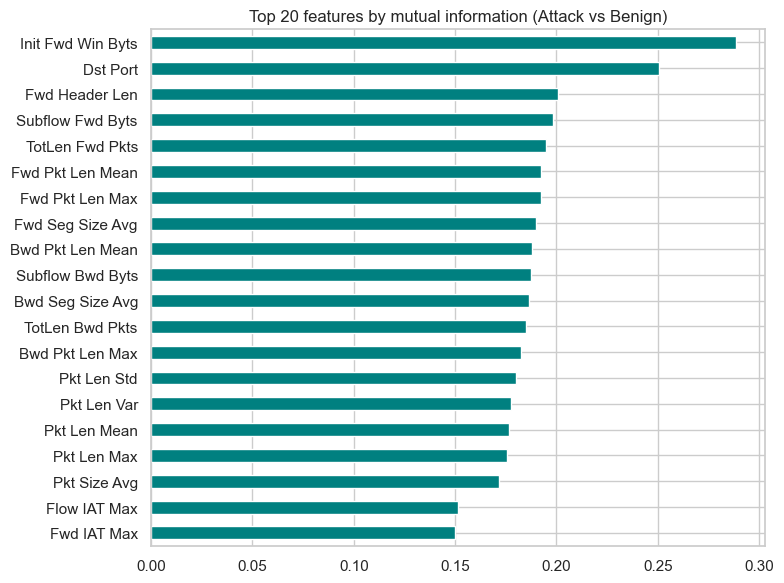
\includegraphics[width=0.49\linewidth]{figures/eda_cse_cic_ids2018_mi.png}\hfill
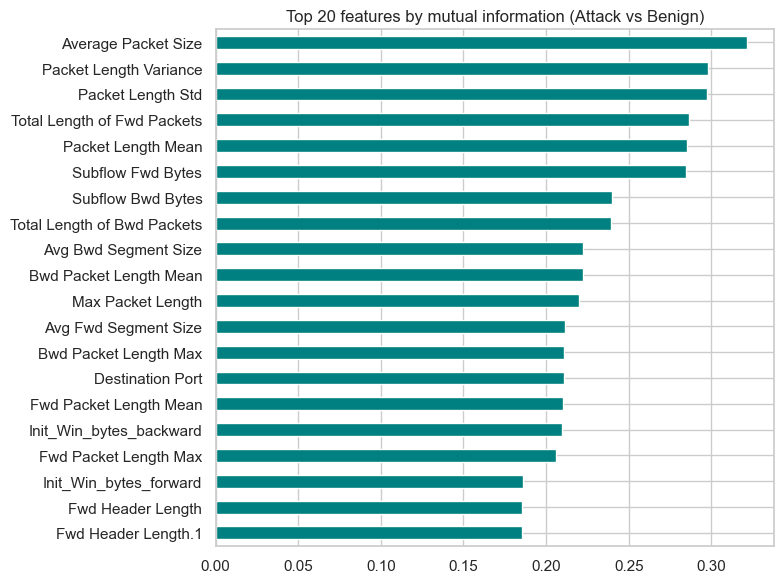
\includegraphics[width=0.49\linewidth]{figures/eda_cic_ids2017_mi.png}
\caption{Top 20 features by mutual information on the raw data. Left: CSE-CIC-IDS2018. Right: CIC-IDS2017 (the
first seven files, before the Wednesday file was added).}
\end{figure}

\begin{figure}[H]
\centering
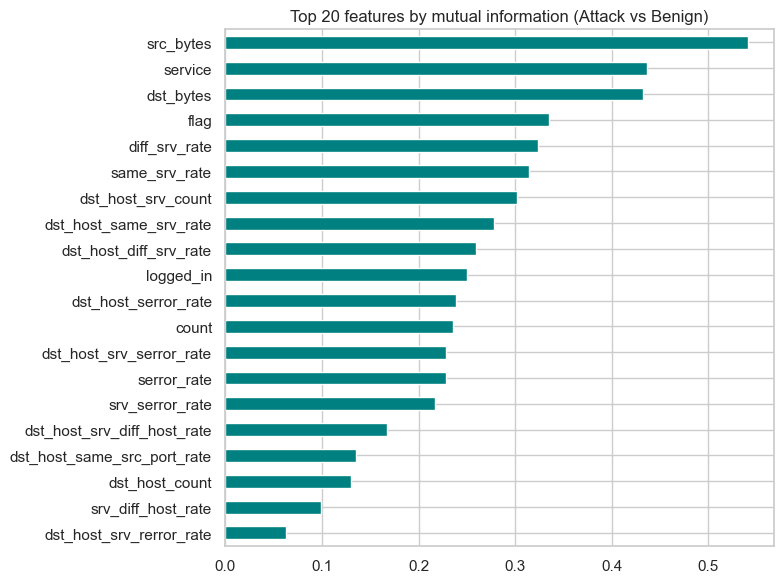
\includegraphics[width=0.49\linewidth]{figures/eda_nsl_kdd_mi.png}\hfill
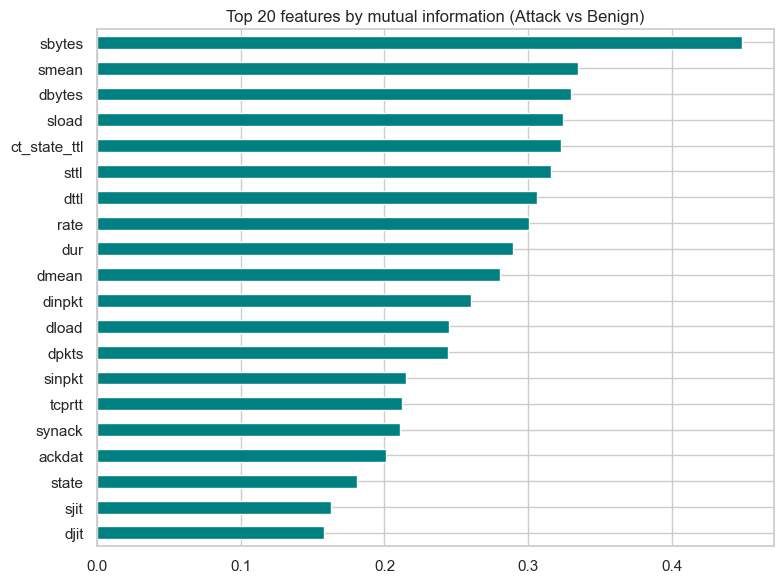
\includegraphics[width=0.49\linewidth]{figures/eda_unsw_nb15_mi.png}
\caption{Top 20 features by mutual information. Left: NSL-KDD. Right: UNSW-NB15.}
\end{figure}


\end{document}
